\section{Target Group}
\begin{figure}[H]
\centering

\includegraphics[scale=0.5]{IKEAInterview.jpg}
%\caption{iPhone game using a gyroscope sensor}
\end{figure}
Good understanding of our target group helps to create good concept - establishing design requirements by answering users special needs and wishes. 
This project is targeting at people who are IKEA shop's customers and who are newly decorating or changing furniture, decor  of their home. This part of research includes two parts - understanding people who has need for application that we develop, and IKEA's target group - people that Ikea attracts  and who are coming to shop for furniture or decor.

There are many ways to segment target audience. Probably most popular is Geographic or Demographic segmentation. In this case we will go deeper and have a look at Psychographics too as we want to know specific needs of customers which will help to design helpful app. 
\subsection{Demographics }
\subsubsection{What is IKEA targeted customer's age ?}
There is no official specific range of age that IKEA is targeting at. Contacting IKEA also did not result in finding out their specific age range. IKEA's targeted group age range is really wide - there are lounges for children, considerations for disabled and old people. At "IKEA'S Accessibility Plan" (Accessibility Plan 2013) they mention that there are consideration to accept people from children to old aged or disabled people. Report even states that staff is trained to help people with disabilities, their equipment and even help-animals. All IKEA shops has mini restaurants where different range of age people can eat. They serve special menus for children, sell wine, and has quick walk-by coffee machines. Assumption can be made that IKEA is trying to appeal to all age range and has not created clear concept design around specific life-cycle stage (examstutor.com, 2015) nor age range. 

However, looking at IKEA's actual customers and considering that in general furniture price is low, we can state that IKEA attracts young people, who cares about expenses. At our first interview with customers we interviewed 10 people and average age was 35 years. Danish people become parents pretty late, on average women give first birth when they are 29 years old (Statistics Denmark 2014). On average Dane man gets married at late age of 35 and 32 as woman. Conclusion can be made that IKEA attracts young people - students, young couples and families, who has less income and priorities of expenses are probably somewhere else as taking care of children or study expenses. It means that we should target at range of age 25-35 which includes, students, young couples and parents.  
\subsection{Psychographics}
Since IKEA is targeting at young people with lower income level, it is possible to do more accurate analysis of social class, lifestyle and personality traits of our target group (Examstutor.com,  2015). According "examstutor" website, social class is categorized in grade class, where IKEA’s targeted customers could be defined as class C1, C2, D or E:
\begin{figure}[H]
\centering
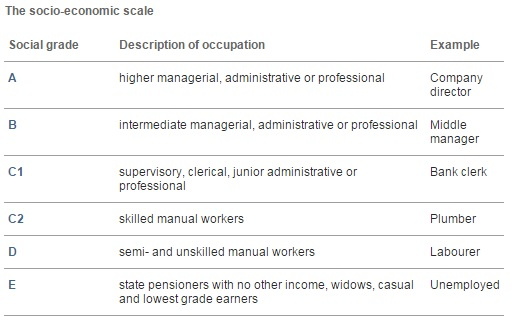
\includegraphics[scale=0.5]{SocialClassDiagram.jpg}
\caption{Scale of the economic classes}
\end{figure}
If most of our target group has lower income level, it would be reasonable to assume that most of IKEA customers does not have expensive gadgets as leading-brand, expensive smartphones. However, our first interview showed that 9 out of 10 have smartphones. Further investigation of finding out which smartphones users have, would be useful to know how optimized an application needs to be for slower mobile devices. 
Analyzing lifestyle traits, means touching upon values, beliefs, interests and opinions. According age, and other statistical information on "Statistic Denmark" it is understandable that IKEA’s customers are busy people - students, young parents and couples, people who are beginning their career life. 
\begin{figure}[H]
\centering
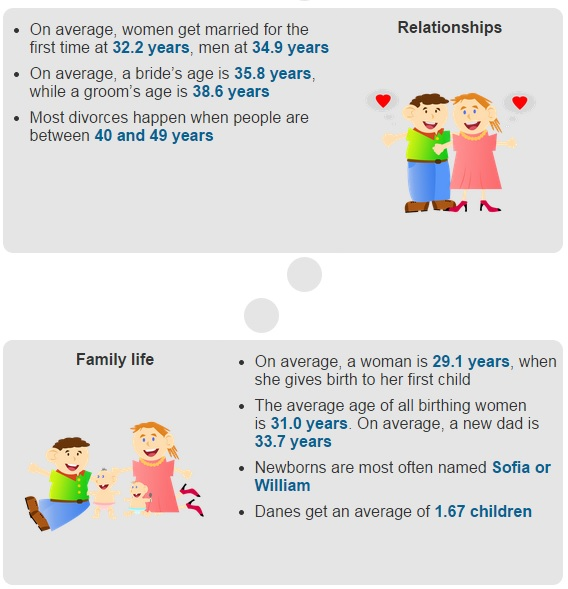
\includegraphics[scale=0.5]{StatiticsDenmark.jpg}
\caption{Relationship statistics}
\end{figure}
statisticsdenmark.com
While interviewing customers we found out that around 50\% count their expenses  while shopping at IKEA. This only would places social class categorization in doubt. However, while interviewing employees of the shop, it was more clear that customers are actually concerned about the price of product - in fact as employess states, price is one of the most common topic to talk with customers. This confirms social class categorization mentioned above. 
\subsection{Digital knowledge}
Marc Prensky in his 2001 article categorizes his understanding of target group to two segments,when it comes to understanding or learning with digital technology. He categorizes them to "digital natives" and "digital immigrants".There are few more categorizations that people use as "Born digital" or "Digital Settlers", so it is common to separate people to "digital knowledge" groups.  Immigrant- is the one who was born and grew up before technology revolution, so for example 65 years old man who did not have all the computers and digital tools or equipment as we do now. This person only adopted to technology at certain age or life point when it was needed. Digital native is the one who grew up in technology era, where he had access for example to Internet, computers, probably experienced one or more ways of learning in digital environment.(Prensky, 2001). However, Prensky notices that time will make everyone a "digital native", as everyone will be born in world full of advanced technology, so old generalization terminology will not be suiting in future. He quotes Albert Einstein - "The problems that exist in the world today cannot be solved by the level of thinking that created them." Prensky later introduces "Digital wisdom" that is more general but suiting in this era.(M. Prensky, 2008). This "tag" is best suiting to our target group - if IKEA's customers are young students or people around 35 years of age it means that target group is on the edge of being called both- if person born in 80s or 90s he/she had a chance to learn or use modern technology, depending on geographical and social class of course. That is why terminology of "Digital wisdom" is useful - we can assume that most of our target group will be with digital wisdom. Therefor most of the targeted users should not have huge problems to start using any digital application.
Interviewing our target group gave us knowledge that users plan and prepare before going to actual shop. 100\% of our interviewed people do some kind of measurements when buying furniture. 10/10 interviewed checked website before going to IKEA and 9/10 are shopping online. 7/10 had planned shopping  the day we interviewed.
\subsection{Target group conclusion}
Our target group are young and busy people - from age of 25-35 who are shopping at IKEA for new furniture or decor. Majority has access to personal smartphone and digital-wisdom in using it’s applications. Our target group are careful with expenses and considering the price, they also tend to know about the product before actually visiting the shop. 


